\documentclass[11pt]{article}
\usepackage[a4paper,margin=23mm]{geometry}
\usepackage[T1]{fontenc}
\usepackage{lmodern,amsmath,amssymb,amsthm,mathtools,microtype,graphicx,booktabs}
\usepackage[colorlinks=true,linkcolor=blue,citecolor=blue,urlcolor=blue]{hyperref}
\newcommand{\HH}{\mathcal H}
\newcommand{\Alg}{\mathcal A}
\newcommand{\CC}{\mathcal K(\HH)}
\newcommand{\Tr}{\operatorname{Tr}}
\newcommand{\dd}{\mathrm d}
\newcommand{\norm}[1]{\left\lVert#1\right\rVert}
\newtheorem{proposition}{Proposition}
\title{Stationary states of the selected Slater algebra\\
\large A compact-ideal classification and the covariant-observable interface}
\author{Alan Day \and Chengheng\thanks{AI research assistant (OpenAI).}}
\date{8 November 2026\quad Local research draft}
\begin{document}\maketitle
\begin{abstract}
The same-disorder Slater transfer has a bounded, purely absolutely
continuous Hamiltonian and a compact selected creation operator.
We identify its norm algebra as continuous functions of the Hamiltonian
plus compact operators. Every stationary state on this algebra factors
through its commutative energy quotient and annihilates all selected
insertions. There is no normal stationary density on the full Type I
closure. We construct finite-time averaged normal states and quantify
their loss of finite-rank signal. A separate exact covariance argument
recovers tracial correlators on microscopic covariant observables,
providing the next route to nontrivial stationary bilocal dynamics.
The conclusions concern a specified algebra, representation and flow;
they are not a no-go statement for de Sitter holography.
\end{abstract}

\section{The physical question and existing input}
Rahman--Susskind distinguish Boltzmann temperature from Hawking
temperature and tomperature, with explicit cosmic/string unit
conversions \cite{RS}. We therefore do not infer a Gibbs density in
our representation from a de Sitter temperature. Rajgadia--Xu
distinguish generic probes from state-adapted dressed probes and
obtain a Type I algebra for the latter \cite[Secs.~4.2, 9.2]{RX}.
The present same-$J$ complex model differs from their matter ensemble.
Our task is to examine the state space of the transfer already derived.

Normal states, invariance and the ordinary Type I Gibbs criterion
are standard \cite[Secs.~8.3--8.6]{D}. The compactness arguments
below are elementary applications, written out to separate normal
states, singular states and changes of observable algebra.

\newpage
\section{Model, units and the norm algebra}
Use the established half-filled Slater construction with standard CAR,
overlapping $p$-body sets and the same Hermitian Gaussian $J$:
\begin{align}
 H_N&=\sqrt{w_N}\sum_{|A|=|B|=p}J_{AB}C_A^\dagger C_B,
 &\mathbb E J_{AB}J_{CD}&=\delta_{AD}\delta_{BC},\\
 M_N^\dagger&=L_N^{-1/2}\sum_{A\subset O^c,B\subset O}J_{AB}C_A^\dagger C_B,
 &h_N&=H_N/\sqrt{w_ND_N},\\
 L_N&=\binom{N/2}{p}^{\!2},
 &D_N&=\binom{N/2}{p}\binom{N/2+p}{p}.
\end{align}
The state is $\varphi_N=\mathbb E\langle O|\,\cdot\,|O\rangle$.
Take $p^2/N\to\lambda>0$, $q=e^{-4\lambda}\in(0,1)$ and
$\hbar=1$. Energies below are dimensionless $h$ energies; physical
string energies multiply by $J_s/\sqrt\lambda$. Times and inverse
temperatures are conjugate to $h$, not cosmic quantities. All
long-time statements follow the double-scaled limit; no uniform
finite-$N$ late-time limit is assumed.

The preceding transfer stage supplies a separable graded GNS space,
a cyclic unit vector $\Omega$, finite-dimensional levels, and
\begin{gather}
 h=J_q\otimes I_{\mathcal P},\qquad
 J_q|n\rangle=\sqrt{[n+1]_q}|n+1\rangle+
                    \sqrt{[n]_q}|n-1\rangle,\\
 M\text{ compact},\qquad Q=MM^\dagger-qM^\dagger M=q^{\mathcal N},
 \qquad Q^r\longrightarrow P_\Omega\quad\text{in norm}.
\end{gather}
Here $\mathcal P$ is the primitive multiplicity space. The standard
$q$-Hermite measure $\mu_q$ is absolutely continuous, positive in
the interior of $I=[-E_*,E_*]$, $E_*=2/\sqrt{1-q}$.
Thus $h$ is purely absolutely continuous on the full joint space,
irrespective of primitive multiplicity. Set $\Alg=C^*(1,h,M)$.

\begin{proposition}
\label{alg}
$\Alg=C^*(h)+\CC$, with unique decompositions $f(h)+K$, and
$\Alg/\CC\simeq C(I)$ by $f(h)+K\mapsto f$.
\end{proposition}
\begin{proof}
$P_\Omega\in\Alg$ by the norm limit above. Products
$A P_\Omega B^*$ with $A,B\in\Alg$ and cyclicity norm-approximate
every rank-one operator, so $\CC\subset\Alg$. Conversely $M\in\CC$.
Every nonempty relatively open spectral interval has an
infinite-dimensional spectral projection. If $f\ne0$ is continuous,
$f(h)$ is bounded below on one such subspace and cannot be compact.
More precisely its essential norm is $\norm{f}_\infty$.
The image of $C^*(h)$ in the Calkin algebra is consequently
isometric and closed. Its inverse image is the closed sum
$C^*(h)+\CC$, proving the assertion.
\end{proof}

\newpage
\section{Normal states and stationary quotient states}
Let $\alpha_t(A)=e^{ith}Ae^{-ith}$. It is norm-continuous since
$h$ is bounded, and preserves $\Alg$ and its compact ideal.

\begin{proposition}\label{normal}
There is no normal stationary state on $B(\HH)$ for $\alpha$.
For every finite real $\beta$, $e^{-\beta h}$ is not trace class.
\end{proposition}
\begin{proof}
A normal stationary state has a positive trace-one density $\rho$
commuting with $h$ \cite{D}. A nonzero positive trace-class operator
has a positive eigenvalue with finite-dimensional eigenspace.
That eigenspace is $h$-invariant. The restriction of self-adjoint
$h$ to it has an eigenvector, contradicting the absence of point
spectrum. Also $e^{-\beta h}\ge e^{-|\beta|E_*}I$ on an
infinite-dimensional space, so its trace diverges.
\end{proof}

This does not exclude singular stationary states. Their restrictions
to the norm algebra can instead be classified exactly.
\begin{proposition}\label{states}
Every stationary state of $\Alg$ is uniquely
\begin{equation}\label{quotient}
 \omega_\nu(f(h)+K)=\int_I f(E)\dd\nu(E),
 \qquad \nu\text{ a probability measure on }I.
\end{equation}
Conversely every such state is stationary. All are tracial and
are $\beta$-KMS for every finite $\beta>0$ (and traces at $\beta=0$).
\end{proposition}
\begin{proof}
The restriction of a positive bounded functional to $\CC$ has
the form $K\mapsto\Tr(\rho_cK)$ with positive trace-class $\rho_c$,
possibly of trace less than one. Stationarity implies
$e^{-ith}\rho_c e^{ith}=\rho_c$, by testing all rank-one $K$.
The previous eigenspace argument forces $\rho_c=0$.
The state therefore factors through the quotient in
Proposition~\ref{alg}; the Riesz representation theorem gives
\eqref{quotient}. The quotient dynamics is the identity and the
quotient is commutative, so these states are tracial and obey
the KMS boundary condition, with a constant analytic function.
\end{proof}

In particular $\omega_\nu(M^\dagger M)=\omega_\nu(MM^\dagger)=0$.
Every finite product of bounded elements of $\Alg$ that contains
an $M$ or $M^\dagger$ insertion is compact, including time-translated
insertions. Its stationary expectation is zero. The GNS algebra
of $\omega_\nu$ is the abelian multiplication algebra $L^\infty(I,\nu)$.
The energy distribution is arbitrary; KMS alone does not choose
$e^{-\beta E}\mu_q/Z$ here. This loss of dynamical information
is stronger than merely failing to normalize an ordinary trace.

\newpage
\section{Weak closure and long-time preparation}
The von Neumann closure of $\Alg$ is $B(\HH)$, but stationary
states of the norm algebra must not be confused with normal states
of that closure. There is also no singular finite-$\beta$ KMS
state on the full $B(\HH)$ for this bounded inner flow.
Indeed, if $\omega$ were one, $h$ lies in its centralizer and
\begin{equation}
 \tau(A)=\frac{\omega(e^{\beta h}A)}{\omega(e^{\beta h})}
\end{equation}
would be a positive normalized trace. Positivity follows by moving
$e^{\beta h/2}$ through the functional. The KMS identity
$\omega(XY)=\omega(Y\alpha_{i\beta}(X))$ gives
$\tau(AB)=\tau(BA)$. Two isometries $V_1,V_2$ with orthogonal
ranges summing to $I$ would then give
$1=\sum_i\tau(V_iV_i^*)=\sum_i\tau(V_i^*V_i)=2$.
This rules out KMS states on the full closure, not arbitrary
singular invariant states. It also explains why a KMS state
on $\Alg$ cannot extend as a KMS state to that closure.

\begin{proposition}\label{limit}
For every normal density $\rho$, as $|t|\to\infty$,
\begin{equation}\label{weak}
 \Tr\bigl(\rho\alpha_t(f(h)+K)\bigr)
 \longrightarrow \int_I f(E)\dd\nu_\rho(E),\qquad
 \nu_\rho(B)=\Tr(\rho P_h(B)).
\end{equation}
This is pointwise weak-* convergence on $\Alg$.
\end{proposition}
\begin{proof}
The scalar spectral measure between any two vectors has an
$L^1$ density, since $h$ is purely absolutely continuous.
The Riemann--Lebesgue lemma gives $e^{-ith}\psi\rightharpoonup0$.
For compact $K$, $K e^{-ith}\psi\to0$ in norm; hence its vector
expectation vanishes. Trace-norm finite-rank approximation of
$\rho$ extends this to all normal densities. The $f(h)$ part
is conserved exactly. This proves \eqref{weak} without time averaging.
\end{proof}

For the previous selected Euclidean preparation
$\psi_\beta=Z_M^{-1/2}e^{-\beta h/2}M^\dagger\Omega$, this yields
\begin{equation}
 \dd\nu_{\psi_\beta}(E)=
 \frac{e^{-\beta E}(1-\sqrt q+\sqrt q E^2)}{Z_M}\dd\mu_q(E).
\end{equation}
Its energy bias survives, while compact selected signals disappear.
The limit has no density operator in this representation. Nor is
convergence claimed for every bounded observable of $B(\HH)$.
The inverse dressing $q^{-\mathcal N/2}M$ is unbounded and is
outside the compact-ideal argument; it cannot be inserted into
these bounded-word statements without new domain and moment control.

\newpage
\section{Finite observation times: an explicit family}
Normal approximately stationary states do exist at finite duration.
For $T>0$ define the trace-norm integral
\begin{equation}
 \rho_T=\frac1{2T}\int_{-T}^T
          e^{-ith}P_\Omega e^{ith}\dd t.
\end{equation}
It is positive of trace one. Comparing two shifted intervals gives
\begin{equation}\label{shift}
 \norm{e^{-iuh}\rho_Te^{iuh}-\rho_T}_1
 \le\min\{2,|u|/T\}.
\end{equation}
The bound follows from the measure of the symmetric difference;
it requires no spectral approximation. Write
$R(t)=\langle\Omega,e^{ith}\Omega\rangle=\int e^{itE}\dd\mu_q(E)$.
Then, exactly in the limiting model,
\begin{align}
 \Tr(\rho_TP_\Omega)&=\frac1T\int_0^T |R(t)|^2\dd t,\label{signal}\\
 \Tr(\rho_T^2)&=\frac1T\int_0^{2T}
                \left(1-\frac{t}{2T}\right)|R(t)|^2\dd t.\label{purity}
\end{align}
The second identity follows by integrating over the difference of
the two times in $[-T,T]^2$. The $q$-Hermite density $r_q(E)$
is bounded on a compact interval for each fixed $q<1$, so
$r_q\in L^2$. Parseval and dominated convergence give
\begin{equation}\label{kappa}
 \kappa_q=\pi\int_I r_q(E)^2\dd E,\qquad
 \Tr(\rho_TP_\Omega)\sim\frac{\kappa_q}{T},\quad
 \Tr(\rho_T^2)\sim\frac{\kappa_q}{T}.
\end{equation}
Thus smaller stationarity defect in \eqref{shift} accompanies
loss of any fixed finite-rank record, rather than convergence to
a trace-class equilibrium. These are sequential limits, first
double scaling and then $T\to\infty$.

For reproducible finite quadrature let $E_j,w_j$ be the eigenvalues
and vacuum weights of an $L$-site $q$-Jacobi matrix. Equations
\eqref{signal}--\eqref{purity} become
\begin{align}
 S_L(T)&=\sum_{jk}w_jw_k\operatorname{sinc}(T(E_j-E_k)),\\
 P_L(T)&=\sum_{jk}w_jw_k\operatorname{sinc}^2(T(E_j-E_k)),
 \qquad \operatorname{sinc}(x)=\sin x/x.
\end{align}
At fixed $L$ their $T\to\infty$ limits are both $\sum_j w_j^2>0$.
This is a discrete quadrature recurrence/pinching effect, not
the nonzero purity of a continuum equilibrium. No finite-$L$
plateau is used to prove \eqref{kappa}.

\newpage
\section{A constructive return to covariant observables}
The failure of selected stationary correlators does not remove
the original bilocal route. Let $\Gamma_m(U)=\wedge^m U$ and let
$B_a(J)$ be jointly $U(N)$-covariant, number-preserving random
operators independent of the fixed reference occupation set $O$:
\begin{equation}
 B_a(U\cdot J)=\Gamma_m(U)B_a(J)\Gamma_m(U)^*.
\end{equation}
The Gaussian law is invariant under the induced action on its
$p$-body indices. For every integrable word $F(J)$ in this family,
possibly including $h_N$ and fixed time evolutions, Schur's lemma
on irreducible $\wedge^m\mathbb C^N$ gives
\begin{equation}\label{schur}
 \mathbb E F(J)=\mathbb E\tau_m(F) I_m,\qquad
 \mathbb E\langle O|F(J)|O\rangle=\mathbb E\tau_m(F(J)),
 \quad \tau_m=\binom Nm^{-1}\Tr_m.
\end{equation}
This extends the H-only equality recorded in the earlier Slater
stage; it is a direct symmetry argument, not a new general theorem.
Products remain covariant, so the equality includes all joint
moments rather than only two-point functions.

The restricted annealed state is tracial and stationary on this
covariant algebra at finite $N$. For integrable Gibbs sandwiches,
\eqref{schur} also gives
\begin{equation}\label{gibbs}
 \frac{\mathbb E\langle O|e^{-\beta h_N/2}F
                           e^{-\beta h_N/2}|O\rangle}
      {\mathbb E\langle O|e^{-\beta h_N}|O\rangle}
 =\frac{\mathbb E\tau_m(e^{-\beta h_N}F)}
             {\mathbb E\tau_m(e^{-\beta h_N})}.
\end{equation}
This is joint annealed normalization, not a disorder average of
samplewise normalized Gibbs states. Finite-$N$ cyclicity gives
the KMS boundary relation. Passage to infinite families requires
the existing moment/time-tail estimates for the actual observables.
Equation~\eqref{schur} is a fixed-sector equality, not a license
to replace the central sector by the full charge sum.

Fixed-$O$ $M_N$ is excluded from this covariance family. Its
suppression in the old tracial state is already visible in
\begin{equation}
 \mathbb E\operatorname{tr}_{\rm full}(M_N^\dagger M_N)=4^{-p},
 \quad
 \mathbb E\tau_{N/2}(M_N^\dagger M_N)
 =\frac{\binom{N-2p}{N/2-p}}{\binom N{N/2}}
 =4^{-p}(1+o(1)).
\end{equation}
Each summand after Gaussian contraction is an occupancy projector
on $2p$ distinct sites. The ratio follows from counting its
allowed occupations. Expanding falling factorials gives the
relative correction $O(p/N+p^3/N^2)$ in the stated double scaling.
The full-trace identity was established previously; the saved
small-system enumeration here checks both normalizations.

\newpage
\section{What a joint enlargement must accomplish}
The covariant family provides a nontrivial stationary candidate
without forcing the selected operator itself to be thermal.
One should construct its joint GNS space with the same microscopic
$M_N$, rather than append an unrelated independent matter probe.
The old $h,M$ cyclic space embeds as a reducing subspace for those
generators whenever the joint limit exists. Compactness of $M$
on that subspace does not imply compactness on the enlarged space;
infinite new multiplicity can change it. Thus the present
classification does not rule out this enlargement.

A useful diagnostic is sharper. Suppose $\mathcal B\subset\Alg$
contains $C^*(h)$ and is invariant under $\alpha$, and a normal
state $\rho$ restricts to a stationary state on $\mathcal B$.
For $B=f(h)+K\in\mathcal B$, also $K\in\mathcal B$.
Stationarity and Proposition~\ref{limit} applied to $K^*K$ imply
$\Tr(\rho K^*K)=0$. Applied to $KB'$ for $B'\in\mathcal B$,
the same reasoning shows that the entire compact part vanishes
in the restricted GNS representation. That representation is
abelian with trivial flow. A covariant family with nonzero
dynamical or noncommutative correlators cannot be represented
this way inside the current norm algebra with the same normal state.
This is a concrete test for the proposed bilocal interface.

CLPW instead change the algebra by adding an observer, imposing
the constraint and selecting a positive-energy corner of a crossed
product; their finite trace is not an ordinary trace on our
$B(\HH)$ \cite[Sec.~2.4]{CLPW}. We do not identify the two
constructions. The present result motivates first completing
the microscopic covariant joint interface within the Susskind
program, before adding further observer structures.

The next calculation should retain one previously constructed
nontrivial covariant bilocal generator $B_N$ and evaluate its
same-$J$ mixed Gram data with $h_N,M_N$, beginning with
\begin{equation}
 \mathbb E\langle O|M_N B_N^*B_N M_N^\dagger|O\rangle,
 \qquad
 \mathbb E\langle O|B_N^*M_N^\dagger M_N B_N|O\rangle.
\end{equation}
Projection onto the existing $h,M$ cyclic sector and the norm
of the residual will determine whether new sectors are required.
These quantities are research targets, not computed claims here.
The microscopic interpretation of the joint grading, spatial
and mass generators, finite-$G$ interactions and horizon entropy
remain open. The present stage fixes the state/algebra choice
that those computations must respect.

\newpage
\section{Diagnostics and reproducibility}
\begin{figure}[h]
\centering
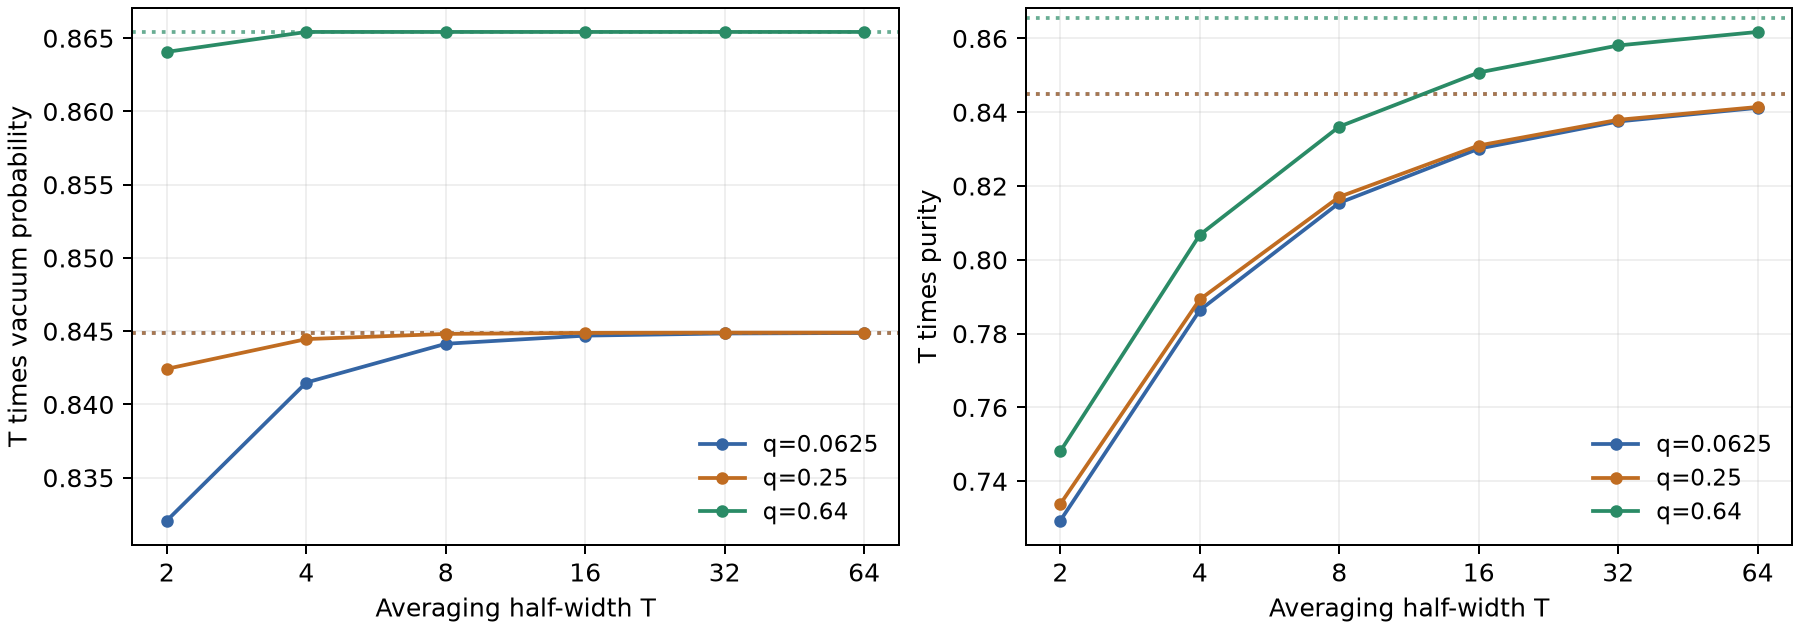
\includegraphics[width=\textwidth]{../../results/susskind-slater-stationary/finite-time-states-layout.png}
\caption{Finite-time normal states. Dotted levels are the independently
integrated $\kappa_q$. Curves use 1100-node quadrature; the theorem
behind the limiting behavior is Parseval, not the numerical fit.}
\end{figure}

The new driver uses $q=0.0625,0.25,0.64$, Jacobi sizes $800,1100$
and $T=2,4,8,16,32,64$, giving 36 quadrature rows. The largest
size-comparison difference is $1.23\times10^{-15}$.
Independent density integrations use $8193/16385$ angle points
and $256/384$ product factors. They give approximately
\begin{equation}
 (\kappa_{0.0625},\kappa_{0.25},\kappa_{0.64})
 =(0.8448905756,\ 0.8449063017,\ 0.8654266760).
\end{equation}
Three direct time-integral comparisons check the sinc and
triangular-kernel formulas. Five finite occupation systems
check the full/central trace factors by enumerating projectors.
The output records relative asymptotic ratios, signed-sum
conditioning, discrete plateaus, parameters, versions and input
hashes. These are float64 diagnostics and exact finite counting,
not interval certification or proofs of the infinite-dimensional
propositions. No old scientific generator was rerun.

\begin{thebibliography}{9}
\bibitem{D} J. Derezi\'nski,
\emph{Introduction to Representations of the Canonical Commutation
and Anticommutation Relations},
\href{https://arxiv.org/abs/math-ph/0511030v2}{arXiv:math-ph/0511030v2},
Secs.~8.3--8.6.
\bibitem{RX} H. Rajgadia and J. Xu,
\emph{Emergent States and Algebras from the Double-Scaling limit of
Pure States in SYK},
\href{https://arxiv.org/abs/2604.14387v3}{arXiv:2604.14387v3}.
\bibitem{RS} A. Rahman and L. Susskind,
\emph{Infinite Temperature is Not So Infinite: The Many Temperatures
of de Sitter Space},
\href{https://arxiv.org/abs/2401.08555v3}{arXiv:2401.08555v3}.
\bibitem{CLPW} V. Chandrasekaran, R. Longo, G. Penington and E. Witten,
\emph{An Algebra of Observables for de Sitter Space},
\href{https://arxiv.org/abs/2206.10780v3}{arXiv:2206.10780v3}.
\end{thebibliography}
\end{document}

